\section{Теория графов}

Графы — это фундаментальное понятие в дискретной математике, и теория графов играет важную роль в изучении различных аспектов их применения. Графы используются для моделирования и анализа множества реальных явлений, таких как сети, маршрутизация, социальные взаимодействия и многое другое.

В этом разделе мы рассмотрим основные понятия теории графов, которые помогут нам заложить базис для дальнейшего изучения этой темы.

\subsection{Основные определения}

Графы обеспечивают эффективное средство для описания бинарных отношений между различными объектами. Чтобы понять эту концепцию, можно взять пример из социальной сети: люди в этой сети представляют собой множество объектов, обозначаемых как $V$. В то же время отношения между этими людьми, такие как подписки или дружба, можно рассматривать как набор бинарных связей. Если объект $v_i$ подписан на объект $v_j$, это означает наличие определенной связи между этими двумя людьми.

Для визуализации графов часто используется графическое представление, в котором объекты изображаются в виде кругов или узлов, а связи между ними – в виде линий или рёбер. Такой способ визуализации помогает лучше понять структуру графа и позволяет легче выявлять взаимосвязи между различными элементами.

В теории графов мы можем классифицировать графы по их структуре и направленности. Граф считается ориентированным, если он содержит непустое множество вершин $V$ и множество отношений или рёбер $E \subset V \times V$, при этом каждое ребро можно трактовать как упорядоченную пару $(v_i, v_j)$. Это означает, что в ориентированном графе направление связи между вершинами имеет значение. В данном случае, если в графе есть ребро из вершины $v_i$ в вершину $v_j$, то может не быть обратного ребра из $v_j$ в $v_i$. Такой граф часто называют "ориентированным графом" или "диграфом".

Если же граф содержит симметричные отношения между вершинами, он называется неориентированным. В неориентированном графе наличие ребра между вершинами $v_i$ и $v_j$ означает, что связь двусторонняя: если есть ребро $(v_i, v_j)$, то автоматически имеется и обратное ребро $(v_j, v_i)$.

Существует также класс графов, называемых смешанными графами. Они обладают одновременно ориентированными и неориентированными рёбрами, что придаёт им более сложную структуру и позволяет описывать более разнообразные ситуации.

На рисунке \ref{fig:digraph} представлен пример различных типов графов, показывающий, как можно визуально различать ориентированные, неориентированные и смешанные графы. Такой подход к изображению графов позволяет легко понять, какой тип отношений присутствует в каждом конкретном случае.

\begin{figure}[H]
	\begin{center}
		 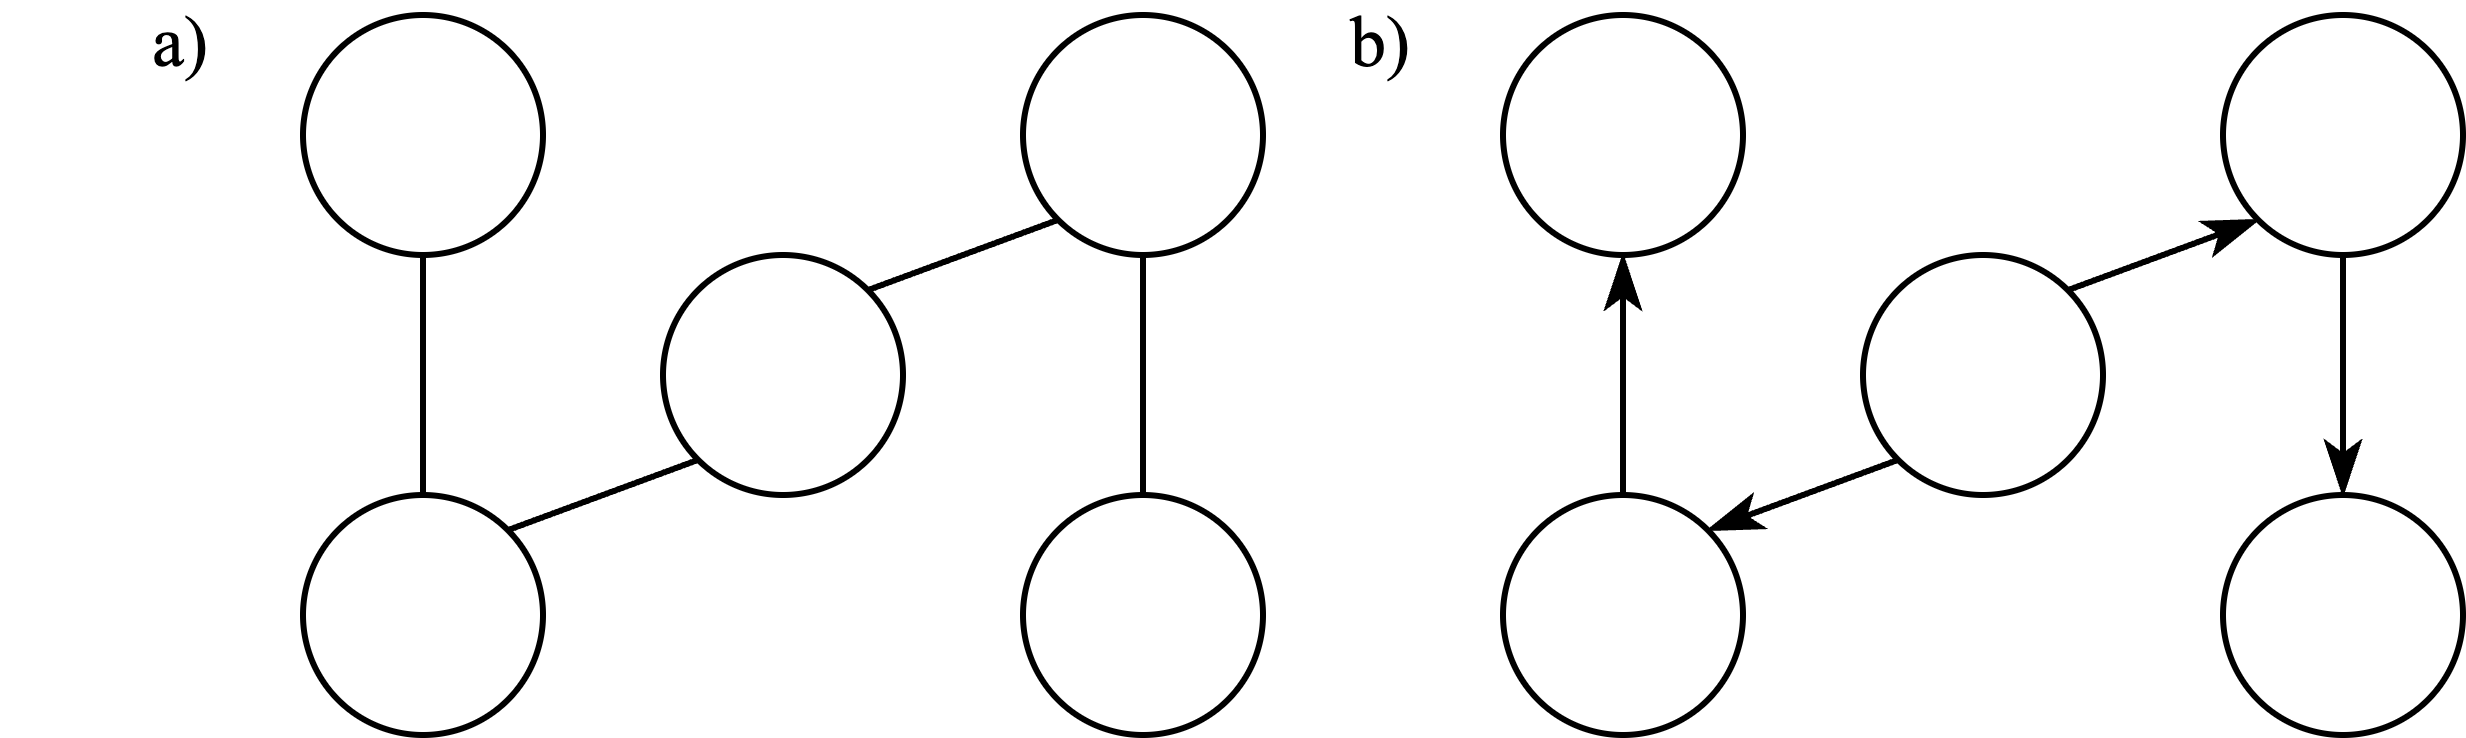
\includegraphics[width=0.9\linewidth]{src/img/1/digraph.png}
		 \caption{Ориентированный граф (a), неориентированный граф (b)}
		\label{fig:digraph}
	\end{center}
\end{figure}

Полный граф — это граф, в котором каждая вершина соединена со всеми другими вершинами. Это означает, что множество рёбер $E$ эквивалентно декартовому произведению множества вершин $V \times V$. В таком графе между любой парой вершин существует прямое отношение или ребро, что создает сеть с максимальной плотностью связей. Полные графы часто используются в различных теоретических моделях и имеют ряд интересных свойств.

Взвешенный граф — это граф, в котором каждому ребру или вершине присваивается некоторый вес или значение. Этот вес может представлять что угодно: от стоимости или длины пути до количества ресурсов или времени, необходимого для преодоления данного ребра или для работы с данной вершиной. Взвешенные графы позволяют анализировать графы с учетом дополнительных параметров и часто используются для задач, связанных с оптимизацией.

Путь в графе — это последовательность рёбер, которая соединяет ряд вершин, начиная с исходной вершины и заканчивая конечной. Формально, путь определяется как набор рёбер $E_1, E_2, \ldots, E_n$, где конечная вершина одного ребра совпадает с начальной вершиной следующего. Путь считается простым, если никакое ребро не повторяется более одного раза. Элементарный путь — это путь, в котором каждая вершина посещается только один раз, что означает отсутствие повторяющихся вершин.

Цикл — это особый тип пути, который начинается и заканчивается в одной и той же вершине. Если граф является направленным, цикл может называться контуром. Циклы важны для выявления повторяющихся процессов или замкнутых систем в графе.

На изображении \ref{fig:path_example} показан пример пути, который является простым, поскольку каждое ребро используется только один раз, но не элементарным, так как центральная вершина посещается дважды. Такие примеры иллюстрируют различия между простыми и элементарными путями и показывают, как они могут применяться в различных контекстах анализа графов.


\begin{figure}[H]
	\begin{center}
		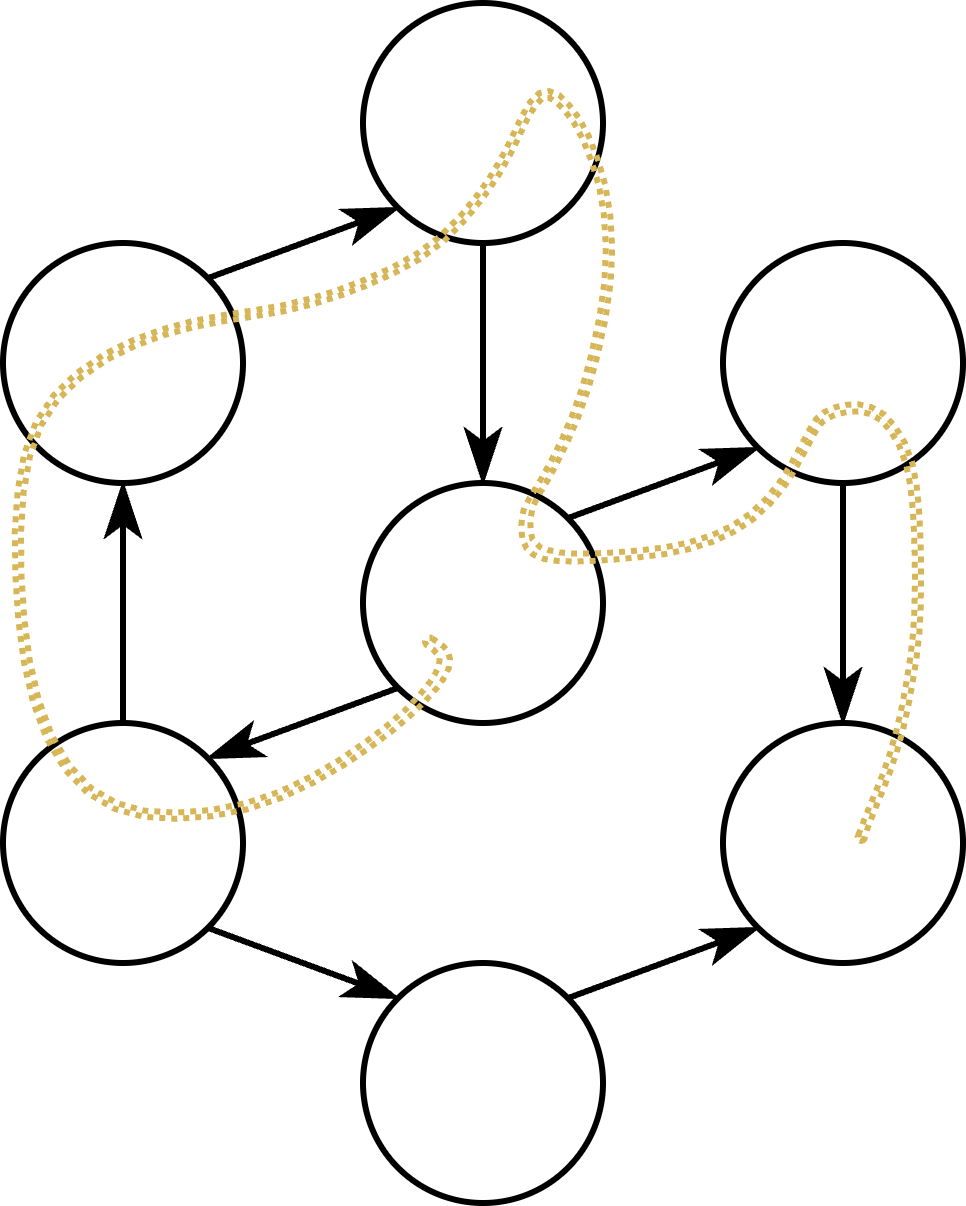
\includegraphics[width=0.40\linewidth]{src/img/1/graph_path.png}
		\caption{Простой, но не элементарный путь в графе}
		\label{fig:path_example}
	\end{center}
\end{figure}

Граф считается связным, если для каждой пары различных вершин в этом графе существует хотя бы один путь, соединяющий их. Это означает, что в связном графе можно переместиться из любой вершины к любой другой, следуя по рёбрам, которые соединяют вершины.

Связность является ключевым свойством графов, которое определяет их структуру и характер. В связном графе все вершины так или иначе соединены друг с другом, даже если путь между ними может проходить через другие промежуточные вершины.

Связные графы часто используются для моделирования систем, в которых элементы имеют некоторую степень взаимодействия или зависимости. Например, в социальной сети связный граф указывает на то, что существует путь коммуникации между любыми двумя участниками сети, даже если они могут быть связаны через нескольких посредников.

Если граф не является связным, то он состоит из нескольких отдельных компонент, каждая из которых представляет собой связный граф. Эти компоненты могут быть изучены отдельно, так как они не имеют связей друг с другом. Исследование связности графов позволяет выявлять изолированные сегменты или группы тесно связанных элементов.


\subsection{Изоморфизм графов}


Изоморфизм в теории графов — это понятие, которое указывает на структурное сходство между графами. Когда говорят, что графы $G_1$ и $G_2$ изоморфны, это означает, что между ними можно установить взаимно однозначное соответствие для вершин и рёбер. Иными словами, если имеется биекция между вершинами двух графов, которая сохраняет структуру рёбер, то такие графы считаются изоморфными.

Изоморфизм графов подразумевает, что их визуальная структура может отличаться, но по сути они идентичны. Например, если у одного графа вершины $A, B, C$ соединены рёбрами в определенной последовательности, то в другом графе можно найти соответствие, в котором другие вершины $X, Y, Z$ имеют те же рёбра в той же последовательности. Изоморфизм позволяет понять, когда два графа, несмотря на различие в именах или представлениях, имеют одинаковую структуру.

Подграфы — это части графа, которые включают некоторую подмножество вершин и рёбер из исходного графа. Если два подграфа из разных графов изоморфны друг другу, то их называют изоморфными подграфами. Такое понятие полезно при анализе сложных графов, когда нужно найти общие структуры или повторяющиеся паттерны.

Двойной изоморфизм подграфов — это ситуация, в которой два разных графа содержат подграфы, которые изоморфны друг другу. Это более широкий концепт, который указывает на то, что в двух графах есть общие структуры, но сами графы при этом могут не быть изоморфными.

Таким образом, изоморфизм и его вариации позволяют исследовать и выявлять структурное сходство в графах, что часто используется в таких областях, как компьютерные науки, биоинформатика и теория сетей.

На изображении \ref{fig:isomorphic_graphs_example} приведен пример двух изоморфных графов.

\begin{figure}[H]
	\begin{center}
		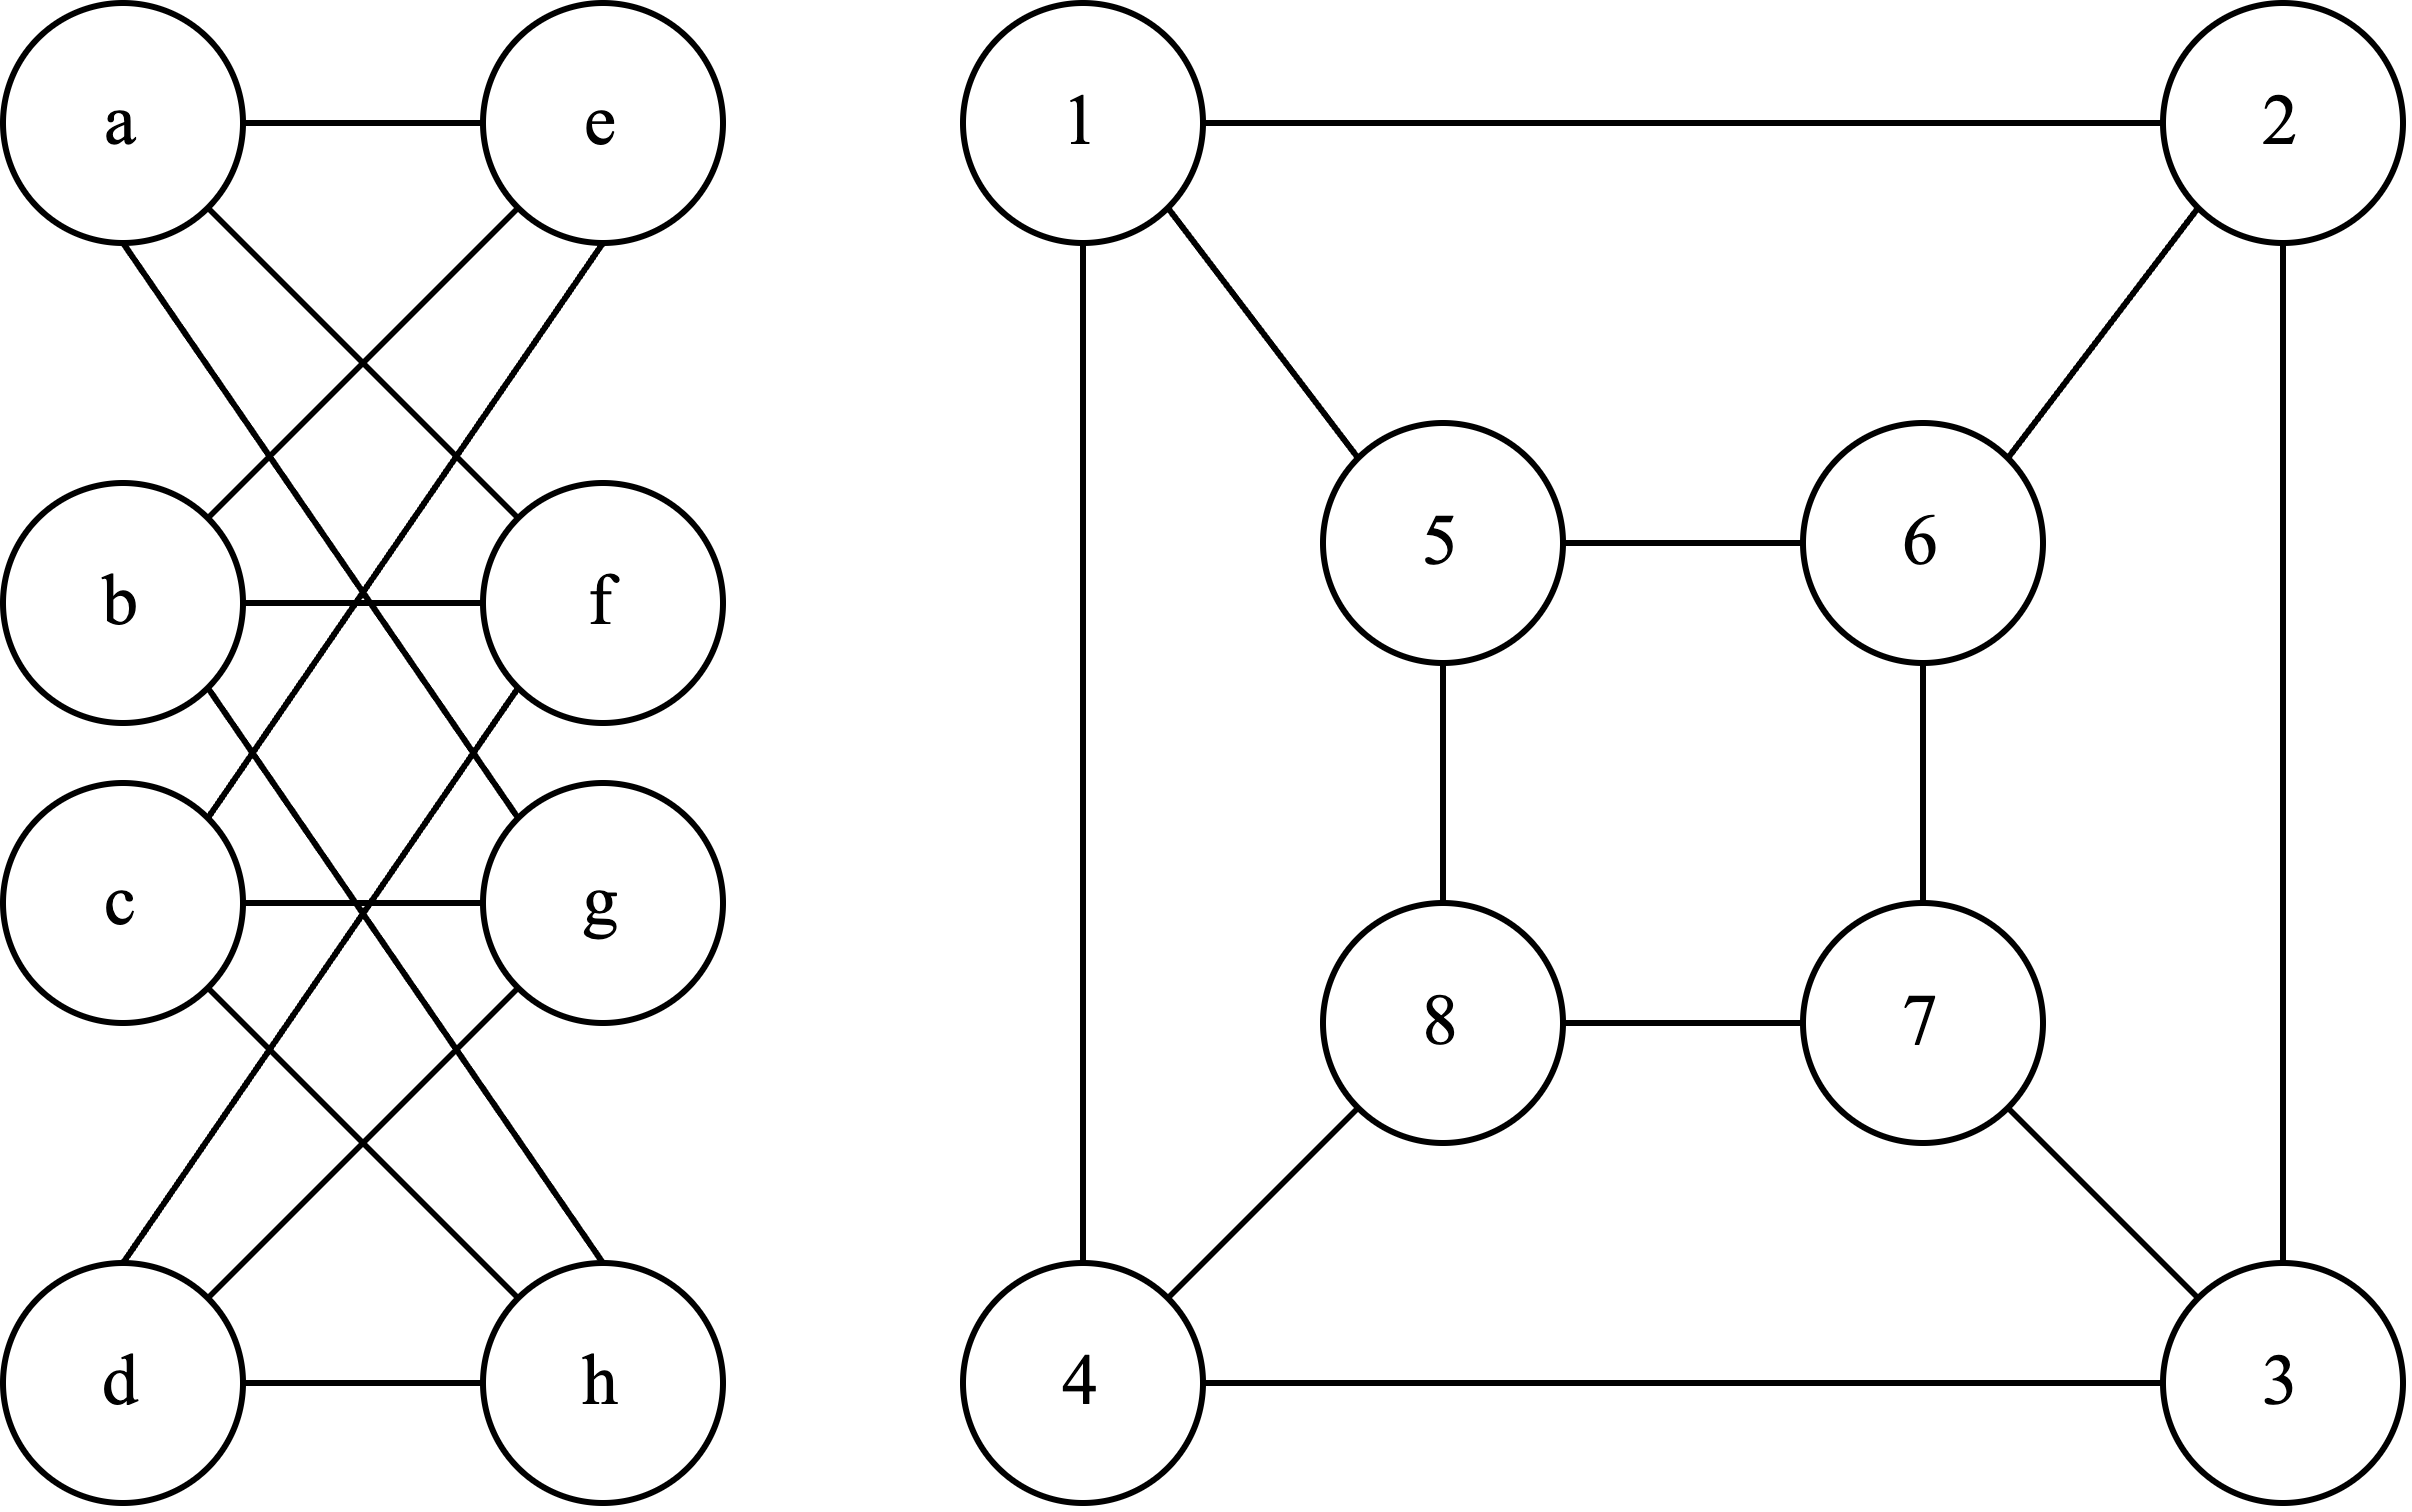
\includegraphics[width=0.7\linewidth]{src/img/1/isomorphic_graphs.png}
		\caption{Пример изоморфных графов}
		\label{fig:isomorphic_graphs_example}
	\end{center}
\end{figure}

\subsection{Деревья}

Деревья представляют собой особый вид графов, которые широко применяются в различных областях информационных технологий, таких как алгоритмы, структуры данных. В этой работе деревья будут служить основой для алгоритмов генерации маршрутов.

Подобно графам, деревья делятся на два класса: ориентированные и неориентированные. Неориентированное дерево — это связный граф, который не содержит простых циклов. Это означает, что если начать обход по дереву из любой вершины, невозможно вернуться к исходной точке, не пройдя по рёбрам назад. Деревья уникальны своей структурой, поскольку они всегда связаны, но не имеют замкнутых путей.

В деревьях есть особые вершины, которые называются листовыми. Листовые вершины — это вершины, которые имеют степень, равную единице, то есть из них выходит только одно ребро. Они представляют собой конечные точки в дереве, и их наличие указывает на то, что это дерево имеет четко определенную структуру без циклов.

Остальные вершины в дереве, из которых выходит более одного ребра, называются внутренними вершинами. Внутренние вершины обеспечивают структуру дерева, соединяя между собой другие вершины и образуя пути, которые могут вести к листовым вершинам.

В целом, деревья обладают рядом полезных свойств, которые делают их ключевым элементом в алгоритмах, особенно тех, что связаны с обработкой данных, маршрутами и поиском путей. Их использование в алгоритмах генерации маршрутов позволяет оптимизировать процесс поиска и обеспечить целостность структуры данных.


\subsection{Клики}


Полный граф — это особый вид графа, в котором каждый узел (вершина) соединён с каждым другим узлом. Это означает, что для любого набора из двух вершин в полном графе всегда существует ребро, соединяющее их. Полные графы могут быть представлены математически как графы, у которых множество рёбер $E$ равно декартовому произведению множества вершин $V \times V$. Визуально, полный граф с $n$ вершинами будет иметь $n(n-1)/2$ рёбер.

Полное множество — это подмножество графа, которое само является полным графом. Другими словами, если выбрать определённое количество вершин из графа, и все они взаимно связаны рёбрами, то такое подмножество можно назвать полным множеством. Полные множества позволяют выделять небольшие полностью связанные участки в больших графах.

Клика — это специальный тип полного множества, который является максимальным. Это значит, что клика представляет собой полное множество, но при этом не существует другого полного множества большего размера, которое включало бы клик. Если добавить любую другую вершину в клик, она перестанет быть полным множеством, так как не будет полностью связанной. Клики полезны в графовых алгоритмах, особенно при анализе социальных сетей или других систем, где важна максимальная взаимосвязь между узлами.

Таким образом, полный граф, полное множество и клика представляют собой концепты, позволяющие описывать степень связи и максимальные подмножества в графах. Они используются в различных алгоритмах и методах анализа графов, в частности при решении задач оптимизации, поиска общих связей и выявления групп узлов с сильной взаимосвязью.

На изображении \ref{fig:clique_example} изображен пример клики.

\begin{figure}[H]
	\begin{center}
		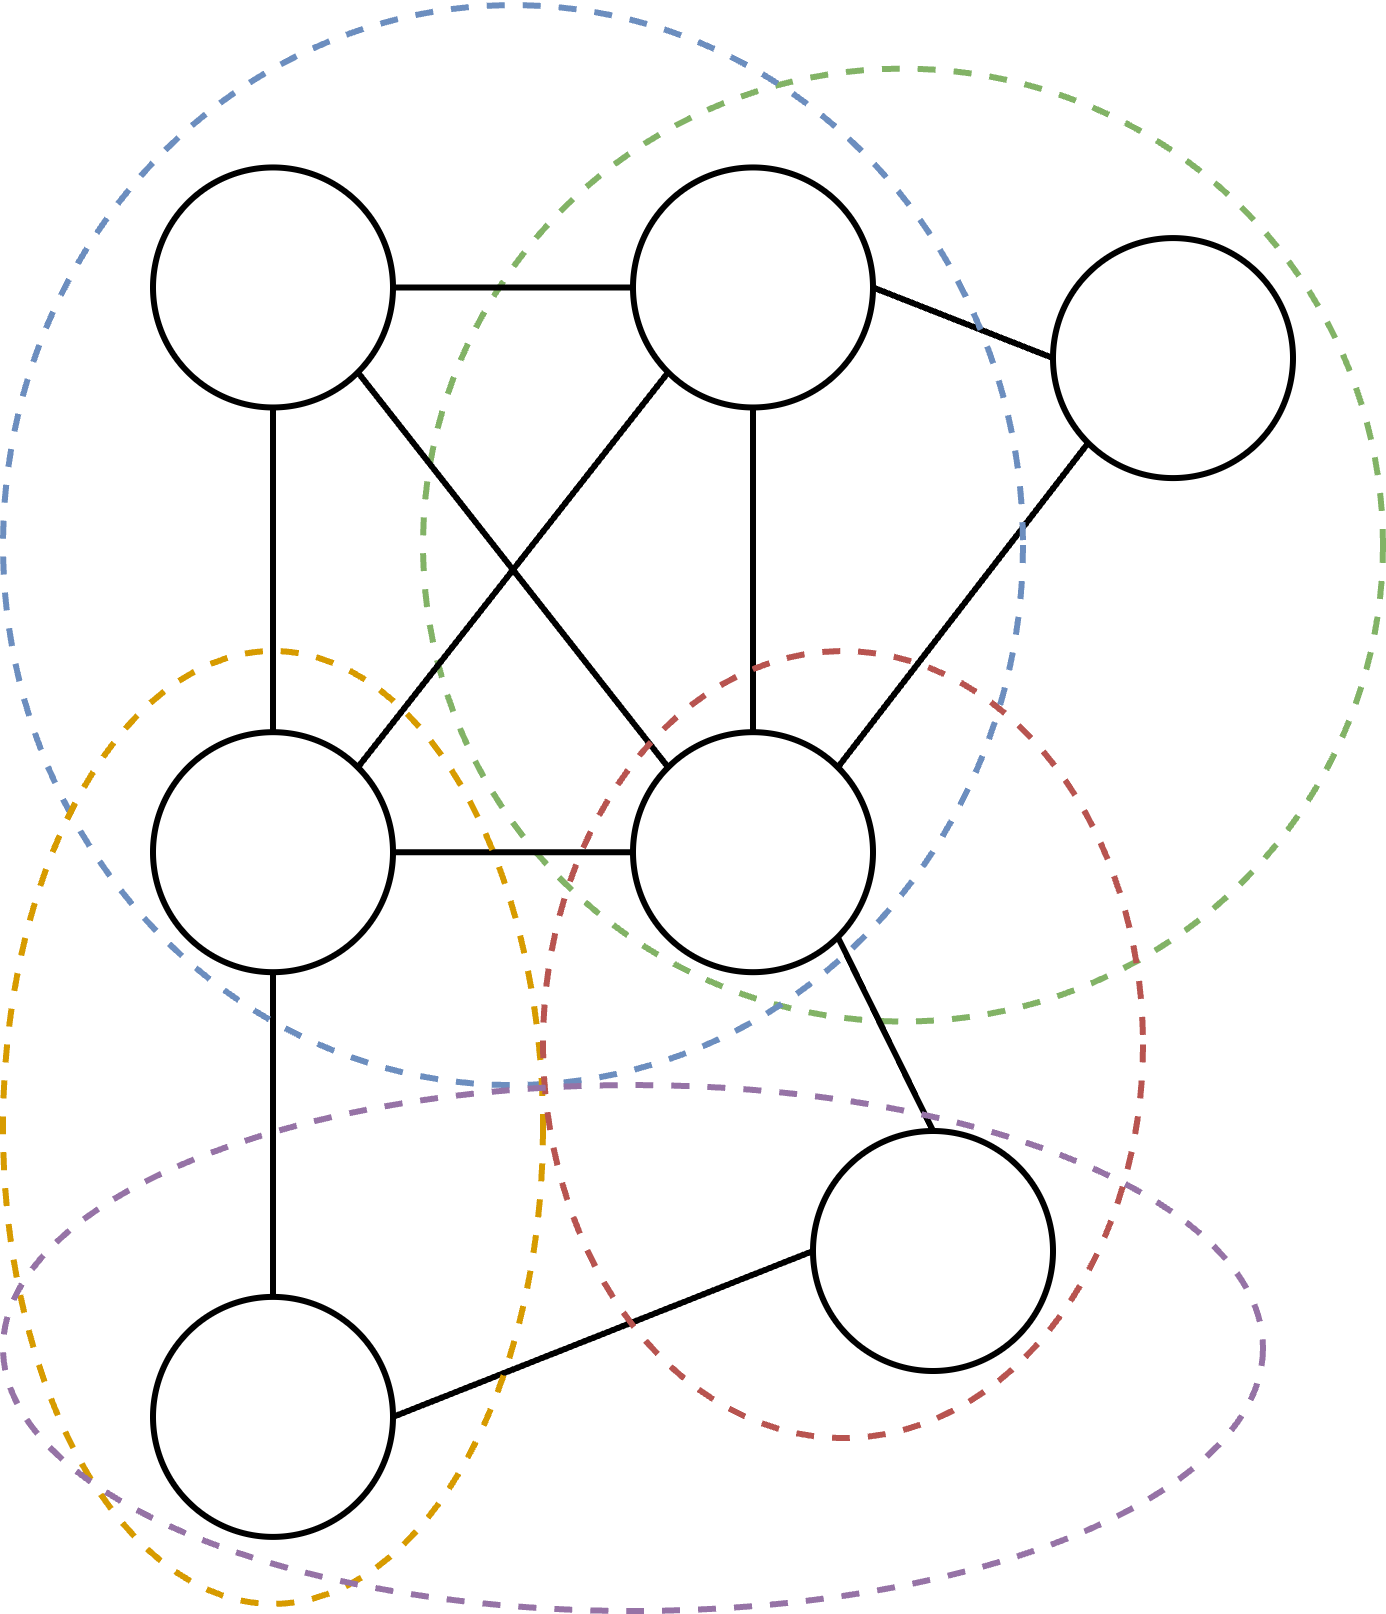
\includegraphics[width=0.40\linewidth]{src/img/1/clique.png}
		\caption{Пример графа с 5 кликами}
		\label{fig:clique_example}
	\end{center}
\end{figure}

В этом графе есть пять клик. Среди них есть клика, состоящая из четырёх вершин, клика с тремя вершинами, а также три клики, в каждой из которых по две вершины.


\subsection{Расстояния на графе}

В теории графов расстояние между двумя вершинами отражает число рёбер, которые нужно пройти, чтобы соединить эти вершины на кратчайшем пути. Это значение позволяет оценить, насколько близко или далеко находятся вершины друг от друга. В невзвешенных графах расстояние определяется просто количеством рёбер на кратчайшем пути. Однако в взвешенных графах, где каждое ребро имеет свой вес, расстояние часто измеряют как сумму весов рёбер на кратчайшем пути.

Эксцентриситет $\epsilon(v)$ вершины $v$ — это максимальное расстояние между данной вершиной и любой другой вершиной графа. Проще говоря, это показатель того, насколько далеко находится одна вершина от самой удаленной вершины в графе. Эксцентриситет позволяет понять, насколько "центральна" или "отдалена" данная вершина относительно всех других вершин.

Радиус $r$ графа — это минимальный эксцентриситет среди всех вершин, то есть $r = \min\limits_{v \in V} \epsilon(v)$. Радиус показывает, насколько компактно расположены вершины графа. Если радиус мал, это указывает на то, что есть вершина, от которой все другие вершины относительно близко. Радиус имеет практическое значение, поскольку он определяет минимальное расстояние, на котором все вершины могут быть связаны.

Диаметр $d$ графа, напротив, — это максимальный эксцентриситет среди всех вершин, то есть $d = \max\limits_{v \in V} \epsilon(v)$. Диаметр представляет собой максимальное расстояние между любыми двумя вершинами в графе. Это значение важно для понимания "размера" графа в терминах наибольшего расстояния между двумя точками. Диаметр может использоваться для определения сложности или глубины структуры графа.

Итак, радиус и диаметр графа позволяют оценить, насколько "разбросаны" или "сконцентрированы" вершины, и применяются в различных анализах, от моделирования сетей до изучения маршрутизации и топологии графов.


\subsection{Раскраска графов}

Раскраска графа — это метод присвоения определенных меток, или "цветов", элементам графа, следуя определенным правилам. Это понятие широко используется в теории графов и находит множество практических применений в различных областях, от планирования и организации до компьютерных алгоритмов и анализа данных.

В самой базовой форме раскраски графа акцент делается на раскраске вершин таким образом, чтобы ни одна пара соседних вершин не имела одинакового цвета. Это означает, что для каждой вершины в графе ее цвет должен быть отличен от цветов ее соседних вершин. Такая раскраска называется раскраской вершин и представляет собой классическую проблему, часто рассматриваемую в контексте задач минимизации использования ресурсов или управления конфликтами.

Раскраска вершин позволяет решить проблемы распределения, где важно избегать конфликтов. Например, в задачах составления расписаний раскраска графа может помочь гарантировать, что определенные события или задачи не пересекаются по времени или ресурсам. В академическом контексте это может быть применено к составлению экзаменационных расписаний, чтобы избежать совпадений у студентов, записанных на те же курсы.

Другие формы раскраски графа включают раскраску рёбер, где цель заключается в том, чтобы рёбра с общими вершинами имели разные цвета. Такая раскраска может быть полезна для планирования или организации сетей, где рёбра представляют собой связи или пути, которые не должны пересекаться.

Сложность задачи раскраски графа зависит от структуры графа и количества доступных цветов. Известно, что раскраска графа — это NP-трудная задача, что означает, что не существует известного полиномиального алгоритма, который мог бы решить её для всех возможных графов. Тем не менее, разработаны эффективные эвристики и специальные алгоритмы, которые позволяют решать задачу раскраски для определенных классов графов или в приближении к оптимальному решению.

Таким образом, раскраска графа — это мощный инструмент, который может использоваться для решения широкого спектра проблем, требующих распределения ресурсов, избегания конфликтов и оптимизации.


\subsection{Эйлеровы и гамильтоновы графы}

Эйлеров путь (или эйлерова цепь) — это путь в графе, который проходит по каждому ребру ровно один раз. Эйлеров путь позволяет проследить весь граф, не возвращаясь на одно и то же ребро. Такой путь важен для задач, связанных с трассировкой, логистикой или, например, в головоломках, где нужно пройти все возможные связи, не повторяясь.

Эйлеров цикл — это разновидность эйлерова пути, который замкнут, то есть начинается и заканчивается в одной и той же вершине. Таким образом, эйлеров цикл позволяет посетить все рёбра, вернувшись в исходную точку. Эйлеров цикл играет важную роль в различных алгоритмах и решениях задач, связанных с круговыми маршрутами или обходом графа.

Полуэйлеров граф — это граф, в котором существует эйлеров путь, но он не замкнут в цикл. Другими словами, в полуэйлеровом графе можно найти путь, который проходит через все рёбра, но начальная и конечная вершины различаются.

Эйлеров граф, в отличие от полуэйлерова, — это граф, в котором можно найти эйлеров цикл. Этот тип графа характеризуется тем, что все вершины имеют чётную степень, что позволяет построить замкнутый путь, проходящий через все рёбра.

Гамильтонов граф — это граф, который содержит гамильтонов цикл. Гамильтонов цикл — это замкнутый путь, который проходит через каждую вершину графа ровно один раз. Этот тип циклов используется в различных задачах, особенно в тех, где нужно организовать последовательное посещение всех вершин графа, как в задачах коммивояжёра или при планировании маршрутов.

Гамильтонов путь — это путь, который проходит через каждую вершину графа ровно один раз, но, в отличие от гамильтонова цикла, он не замкнут. Этот путь может начинаться и заканчиваться в разных точках, и он важен для задач, где нужно пройти через все вершины, не возвращаясь к началу.

Гамильтонов цикл имеет применение в криптографии, особенно в системах протоколов с нулевым разглашением, где он используется для доказательства определённых свойств без раскрытия дополнительных данных.

Эти понятия — эйлеров путь, эйлеров цикл, гамильтонов граф, гамильтонов путь и гамильтонов цикл — важны в теории графов и находят применение в различных практических задачах, от маршрутизации и логистики до криптографии и анализа сетей.

\subsection{Кратчкайшие пути на графе}

Задача о кратчайшем пути в теории графов представляет собой поиск пути между двумя вершинами (или узлами) в графе таким образом, чтобы минимизировать суммарный вес рёбер, по которым проходит этот путь. Вес рёбер может быть различным в зависимости от контекста задачи: длина, стоимость, время, пропускная способность и другие параметры, характеризующие связи в графе.

Этот концепт имеет широкое применение в реальных задачах, таких как навигация, логистика, маршрутизация в компьютерных сетях и многое другое. Например, проблема поиска кратчайшего пути между двумя пересечениями на дорожной карте может быть представлена как задача о кратчайшем пути в графе. В этом случае вершины графа соответствуют пересечениям или точкам интереса, а рёбра представляют собой дорожные сегменты, взвешенные по их длине или времени, необходимому для прохождения.

Задача о кратчайшем пути может быть решена для различных типов графов, включая неориентированные, направленные или смешанные графы. В неориентированных графах порядок рёбер не имеет значения, и связь между двумя вершинами двусторонняя. Напротив, в направленных графах рёбра имеют определённое направление, и для поиска пути нужно учитывать, чтобы все последовательные вершины были соединены соответствующими направленными рёбрами.

Для решения задачи о кратчайшем пути в теории графов существует несколько широко известных алгоритмов, каждый из которых предназначен для разных типов графов и имеет свои преимущества в зависимости от структуры и характера задачи. Давайте рассмотрим основные алгоритмы для поиска кратчайшего пути и их особенности.

Алгоритм Дейкстры предназначен для решения задачи о кратчайшем пути из одного источника в графах с неотрицательным весом рёбер. Этот алгоритм работает по принципу жадного выбора, постепенно увеличивая область охвата, чтобы найти кратчайшие пути. Он обычно используется для задач маршрутизации, так как гарантирует нахождение кратчайшего пути в графах без отрицательных рёбер.

Алгоритм Беллмана–Форда может решать задачу о кратчайшем пути из одного источника, даже если веса рёбер могут быть отрицательными. Этот алгоритм выполняет несколько проходов по рёбрам, корректируя веса путей, чтобы найти оптимальный маршрут. Он особенно полезен, если граф может содержать отрицательные рёбра, хотя и может работать медленнее, чем Дейкстра в графах с неотрицательными рёбрами.

Алгоритм A* решает задачу о кратчайшем пути между двумя конкретными вершинами, используя эвристику для ускорения поиска. Этот алгоритм применяет оценку "расстояния", чтобы приоритетно искать пути, которые вероятно ведут к цели. A* широко используется в задачах, где необходимо быстро находить кратчайшие пути, особенно в контекстах искусственного интеллекта и игровых приложениях.

Алгоритм Флойда–Варшалла предназначен для решения задачи о кратчайшем пути между всеми парами вершин в графе. Он использует динамическое программирование для построения матрицы кратчайших путей между всеми возможными парами. Этот алгоритм особенно полезен, когда необходимо найти кратчайшие пути между всеми вершинами, хотя может быть менее эффективен в разреженных графах.

Алгоритм Джонсона также решает задачу поиска кратчайшего пути между всеми парами вершин, но более оптимизирован для разреженных графов. Он сочетает в себе элементы алгоритма Беллмана–Форда и алгоритма Дейкстры, что позволяет ему быть эффективнее при работе с графами, где рёбер существенно меньше, чем вершин.

Алгоритм Витерби предназначен для решения задачи о кратчайшем стохастическом пути, учитывающего вероятностный вес каждого узла. Этот алгоритм применяется в задачах обработки сигналов и анализа последовательностей, где к весам рёбер добавляется элемент вероятности.

Таким образом, каждый из этих алгоритмов имеет своё уникальное применение в теории графов, позволяя решать задачи о кратчайшем пути в различных контекстах, от маршрутизации и планирования до искусственного интеллекта и анализа данных.

Задача о кратчайшем пути представляет собой важную концепцию в теории графов, находящую широкое применение в задачах оптимизации, планирования, маршрутизации и других областях. Решения этой задачи позволяют находить наиболее эффективные пути в различных сетях и графовых структурах, будь то в реальном мире или в абстрактных моделях.










Дорожная сеть представляет собой граф, где узлы обозначают дорожные развязки или перекрёстки, а рёбра — сегменты дорог между этими узлами. В таких графах вес рёбер обычно отражает характеристики дорожных сегментов, такие как длина, время прохождения или стоимость. Это позволяет моделировать транспортные системы и находить оптимальные маршруты в реальном мире.

Особенность дорожных графов заключается в том, что они могут включать рёбра с разными уровнями значимости. Например, некоторые рёбра могут представлять автомагистрали или главные дороги, которые предпочтительны для дальних поездок. Другие рёбра могут символизировать локальные дороги или улицы с односторонним движением. Для моделирования направленных улиц используются направленные рёбра, что обеспечивает реалистичное представление транспортной инфраструктуры.

Эти различия в значимости рёбер привели к введению концепции "размерности шоссе" (highway dimension). Размерность шоссе — это параметр, который отражает, насколько дорожная сеть структурирована таким образом, что определённые рёбра, такие как автомагистрали, играют ключевую роль в обеспечении дальних маршрутов. Иными словами, дорожные сети с низкой размерностью шоссе имеют чётко определённые пути, которые используются для дальних поездок, в то время как сети с высокой размерностью шоссе более хаотичны.

Использование понятия размерности шоссе позволяет создавать эффективные алгоритмы для поиска кратчайшего пути. Такие алгоритмы учитывают структуру дорожной сети и могут находить оптимальные маршруты быстрее, чем в общих графах. Эти алгоритмы часто применяют различные техники, такие как иерархическое разбиение графа, конденсация сетей и другие методы, чтобы ускорить процесс поиска кратчайшего пути.

Примеры таких алгоритмов включают техники, основанные на иерархии дорожных сетей, алгоритмы сокращения графа (graph contraction), а также алгоритмы с использованием шаблонов или "карманов", позволяющие быстро находить кратчайшие пути. Эти методы широко применяются в системах навигации, городском планировании, логистике и других областях, где важно быстро находить оптимальные маршруты в сложных сетях.







Транспортная сеть в реальных условиях часто обладает стохастическими и временными характеристиками, которые отражают неопределенность и изменчивость в реальной дорожной обстановке. В отличие от детерминированных моделей, которые предполагают фиксированное время в пути между двумя точками, стохастические модели учитывают возможность изменений в зависимости от различных факторов.

Одним из ключевых аспектов, влияющих на время в пути, является колебание спроса на транспортные услуги. В часы пик, когда большое количество людей одновременно передвигаются по городу или транспортной сети, время в пути может значительно увеличиваться. Матричная модель "отправление-пункт назначения" (origin-destination matrix) может помочь проиллюстрировать, как перемещаются люди в течение дня, но она зачастую не учитывает стохастические колебания в спросе.

Кроме колебаний спроса, стохастические сети, зависящие от времени (STD), включают в себя дополнительные случайные факторы, такие как рабочие зоны, плохие погодные условия, несчастные случаи и поломки транспортных средств. Все эти элементы могут существенно повлиять на время в пути, делая его непредсказуемым. В связи с этим использование STD-моделей для представления транспортных сетей является более реалистичным и точным.

STD-модели могут учитывать вариативность времени в пути, отражая вероятностные распределения, а не фиксированные значения. Это позволяет использовать алгоритмы для поиска кратчайшего пути, которые принимают во внимание диапазон возможных времён в пути, а также вероятность различных событий, которые могут возникнуть на маршруте.

В реальных транспортных системах использование STD-моделей позволяет более эффективно управлять движением, прогнозировать задержки и оптимизировать маршруты. В системах интеллектуального транспорта, навигационных приложениях и других технологиях, связанных с планированием маршрутов, эти модели играют ключевую роль в обеспечении надёжности и эффективности.

В итоге, стохастические сети, зависящие от времени, предоставляют более реалистичное представление о том, как работает транспортная система, и позволяют разрабатывать алгоритмы, которые лучше адаптируются к реальным условиям и изменениям на дорогах.






Оптимизация пути в стохастических дорожных сетях представляет собой сложную задачу, поскольку неопределенность и изменчивость могут существенно влиять на конечные результаты. Традиционный подход к поиску оптимального пути обычно фокусируется на минимизации ожидаемого времени в пути, что предполагает, что среднее значение времени в пути является оптимальным критерием. Такой подход, хотя и позволяет использовать многие алгоритмы, применяемые в детерминированных сетях, не всегда отражает реальную динамику стохастических сетей.

Основное преимущество поиска пути с минимальным ожидаемым временем в стохастической сети заключается в простоте. Алгоритмы, такие как алгоритм Дейкстры или Беллмана-Форда, могут быть адаптированы для работы в стохастической среде, при этом взвешенные рёбра могут отражать среднее время прохождения. Однако этот подход имеет существенный недостаток: он не учитывает изменчивость или вариативность времени в пути. Это может привести к тому, что путь с минимальным ожидаемым временем окажется ненадежным, поскольку даже небольшие изменения или случайные события могут значительно повлиять на время в пути.

Для решения этой проблемы некоторые исследователи предлагают использовать распределение времени в пути вместо его ожидаемого значения. Такой подход учитывает вероятность различных задержек или отклонений от стандартного времени в пути. Здесь применяются методы стохастической оптимизации, которые учитывают возможные колебания в времени в пути. Одним из подходов является стохастическое динамическое программирование, которое позволяет найти кратчайшие пути, учитывая вероятностные характеристики дорожной сети.

Концепция надёжности времени в пути стала важным элементом в транспортных исследованиях. Она отражает степень вариативности времени в пути: чем больше изменчивость, тем меньше надёжность. В контексте стохастических сетей надёжность времени в пути указывает на вероятность того, что время в пути будет находиться в определённом диапазоне. Если изменчивость высока, то надёжность низка, так как труднее предсказать, сколько времени займёт путь.

Исследования в этой области продолжают развиваться, стремясь найти баланс между оптимизацией и надёжностью. Более сложные алгоритмы, которые учитывают вероятность и изменчивость, позволяют разрабатывать более устойчивые маршруты и стратегии планирования, особенно в условиях реальных дорожных сетей, подверженных различным случайным факторам.






Для более точного учета надежности времени в пути при неопределенности в стохастических дорожных сетях предложены два основных альтернативных подхода к определению оптимального пути. Оба этих подхода стремятся учесть вариативность времени в пути и обеспечить более надежные маршруты.

Наиболее надежный путь - этот подход фокусируется на максимизации вероятности прибытия к месту назначения вовремя или даже раньше заданного бюджета времени в пути. То есть, он стремится найти путь, который с наибольшей вероятностью позволит достичь пункта назначения в течение определенного времени. Этот подход особенно полезен, когда есть ограничения на время прибытия или фиксированный временной бюджет, который необходимо соблюдать.

Наиболее надежный путь часто применяется в ситуациях, где опоздание может иметь серьезные последствия, таких как авиаперелеты, доставка товаров, или расписания общественного транспорта. Такой подход может использоваться для нахождения маршрутов, которые минимизируют риск опозданий, даже если эти маршруты не являются самыми короткими по времени в среднем.

$\alpha$-надежный путь подход, наоборот, стремится минимизировать бюджет времени в пути, который необходим для достижения заранее заданной вероятности прибытия вовремя. Таким образом, вместо того чтобы фиксировать время в пути и искать путь, который с наибольшей вероятностью уложится в этот бюджет, $\alpha$-надежный путь фиксирует вероятность и ищет путь, который минимизирует максимальное время в пути, позволяющее достичь этой вероятности.

Такой подход удобен, когда важнее обеспечить высокую надежность при разумных затратах времени. Например, если нужно гарантировать $95\%$ вероятность прибытия к определенному времени, $\alpha$-надежный путь позволяет определить, сколько времени в запасе нужно иметь, чтобы достичь этой вероятности.

Оба подхода позволяют исследовать стохастические дорожные сети с учётом неопределённости и изменчивости времени в пути. Наиболее надёжный путь может быть предпочтительным, когда время является критическим фактором, и минимизация риска опоздания является основной задачей. $\alpha$-надежный путь полезен, когда необходимо балансировать между надёжностью и эффективностью, минимизируя время в пути, но сохраняя при этом заданную вероятность своевременного прибытия. Оба этих подхода расширяют возможности анализа и оптимизации в условиях неопределенности в транспортных сетях.



\section{Вероятностные модели}



\subsection{Байесовсеие классификаторы}

\subsection{Марковские цепи}


Марковские цепи являются статистическими моделями, которые можно представить в виде графа. Эти модели часто используются для отображения процессов, которые развиваются со временем и подвержены случайным изменениям. Основная идея марковских цепей заключается в том, что процесс имеет множество состояний, а переходы между этими состояниями зависят только от текущего состояния, а не от всей предыдущей истории. Это свойство известно как "марковское свойство".

Марковская цепь может быть представлена как конечный автомат, у которого есть множество состояний $q_1, q_2, \ldots, q_n$. Переходы между этими состояниями считаются стохастическими, что означает, что они определяются вероятностями. Если существует переход из состояния $q_a$ в состояние $q_b$, то вероятность такого перехода можно выразить как $P(S_t = q_b | S_{t - 1} = q_a)$. Здесь $S_t$ обозначает состояние процесса в момент времени $t$, а $S_{t - 1}$ — состояние в предыдущий момент времени.

Время в марковских цепях дискретное, то есть изменение состояний происходит в определенные моменты времени, которые можно обозначить как $t = 1, 2, 3, \ldots$. Дискретная структура времени позволяет использовать марковские цепи для моделирования процессов, которые изменяются по четким временным интервалам.

Марковские цепи имеют множество применений, включая моделирование систем, где вероятности переходов между состояниями зависят от предыдущего состояния. Например, они широко используются в анализе запасов, теории очередей, анализе цепочек поставок, биологии, экономике, робототехнике и искусственном интеллекте. Кроме того, марковские цепи служат основой для многих алгоритмов машинного обучения и обработки естественного языка, где они помогают предсказывать последовательности событий или состояния системы.

Для описания марковской цепи часто используется матрица переходов, в которой каждый элемент $(i, j)$ представляет собой вероятность перехода из состояния $q_i$ в состояние $q_j$. Эта матрица называется стохастической, поскольку сумма всех вероятностей в каждой строке должна быть равна 1. Используя такую матрицу, можно анализировать и прогнозировать поведение марковской цепи в долгосрочной перспективе, определять стационарные состояния, находить вероятности переходов в различные состояния и многое другое.

Чтобы формально определить марковскую цепь, требуется указать несколько ключевых элементов:

\begin{itemize}
	\item множество состояний $Q = \{q_1, q_2, \cdots, q_n\}$. Это множество включает все возможные состояния, в которых может находиться система. В зависимости от конкретной задачи, эти состояния могут представлять различные категории, события или положения системы;
	\item множество априорных вероятностей $\Pi = \{ \pi_1, \pi_2, \cdots, \pi_n \}$, $\pi_i = P(S_t = q_ii)$ Эти вероятности отражают начальное распределение состояний, то есть вероятность того, что система начнет в состоянии $q_i$. Каждая априорная вероятность $\pi_i$ определяет вероятность того, что в момент времени $t$ система будет находиться в состоянии $q_i$. Сумма всех априорных вероятностей должна быть равна 1, то есть $\sum_{i=1}^{n} \pi_i = 1$;
	\item матрица вероятностей переходов $A = \left(a_{ij}\right)|_{i=\overline{1,n}}^{j=\overline{1,n}}$, $a_{ij} = P(S_t = q_j | S_{t-1} = q_i)$. Эта матрица определяет вероятности переходов между состояниями. Элемент $a_{ij}$ обозначает вероятность того, что система перейдет из состояния $q_i$ в состояние $q_j$ в следующий момент времени, то есть $P(S_t = q_j | S_{t-1} = q_i)$. В каждой строке матрицы суммы всех элементов должны быть равны 1, что указывает на то, что сумма всех вероятностей переходов из одного состояния к другим составляет 100\%.
\end{itemize}

Таким образом, марковская цепь определяет систему, в которой вероятности переходов между состояниями определяются только текущим состоянием, а не предыдущей историей. Этот формализм используется для моделирования и анализа процессов, которые обладают свойством "марковской памяти", где будущее состояние зависит только от настоящего.

\subsection{Скрытые марковские модели}

Для более детального рассмотрения концепции марковских цепей, применим их к задаче прогнозирования погоды. Рассмотрим ситуацию, когда в определенном месте климатические условия могут быть сведены к четырем основным состояниям: солнечный день, облачный день, дождливый день и день с грозой. Предположим, что погода на текущий день зависит исключительно от состояния погоды на предыдущий день. Это ключевой принцип марковских цепей — каждое состояние определяет вероятности перехода к другим состояниям, без учета предыстории. Такой подход позволяет создавать простые, но эффективные модели для прогнозирования.

Начнем с заданных априорных вероятностей. Эти вероятности описывают начальное состояние системы, то есть какую погоду можно ожидать без дополнительной информации. Пусть вероятность солнечного дня равна 0.2, облачного — 0.5, дождливого — 0.2, а вероятность грозы — 0.1. Теперь, определив начальные условия, можно перейти к матрице переходов. Эта матрица показывает вероятность перехода из одного погодного состояния в другое:

\begin{center}
	\begin{tabular}{|l|c|c|c|c|}
		\hline
		\textbf{} & Ясно & Облачно & Дождь & Гроза \\ \hline
		Ясно      & 0.6  & 0.4     & 0.2   & 0.05  \\ \hline
		Облачно   & 0.3  & 0.7     & 0.2   & 0.1   \\ \hline
		Дождь     & 0.3  & 0.3     & 0.2   & 0.2   \\ \hline
		Гроза     & 0.4  & 0.3     & 0.3   & 0.1   \\ \hline
	\end{tabular}
\end{center}
\captionof{table}{Матрица вероятностей смены погоды}
\label{tab:pogoda_prob}

Матрицу переходов между состояниями можно изобразить в виде графа как на изображении 

\begin{figure}[H]
	\begin{center}
		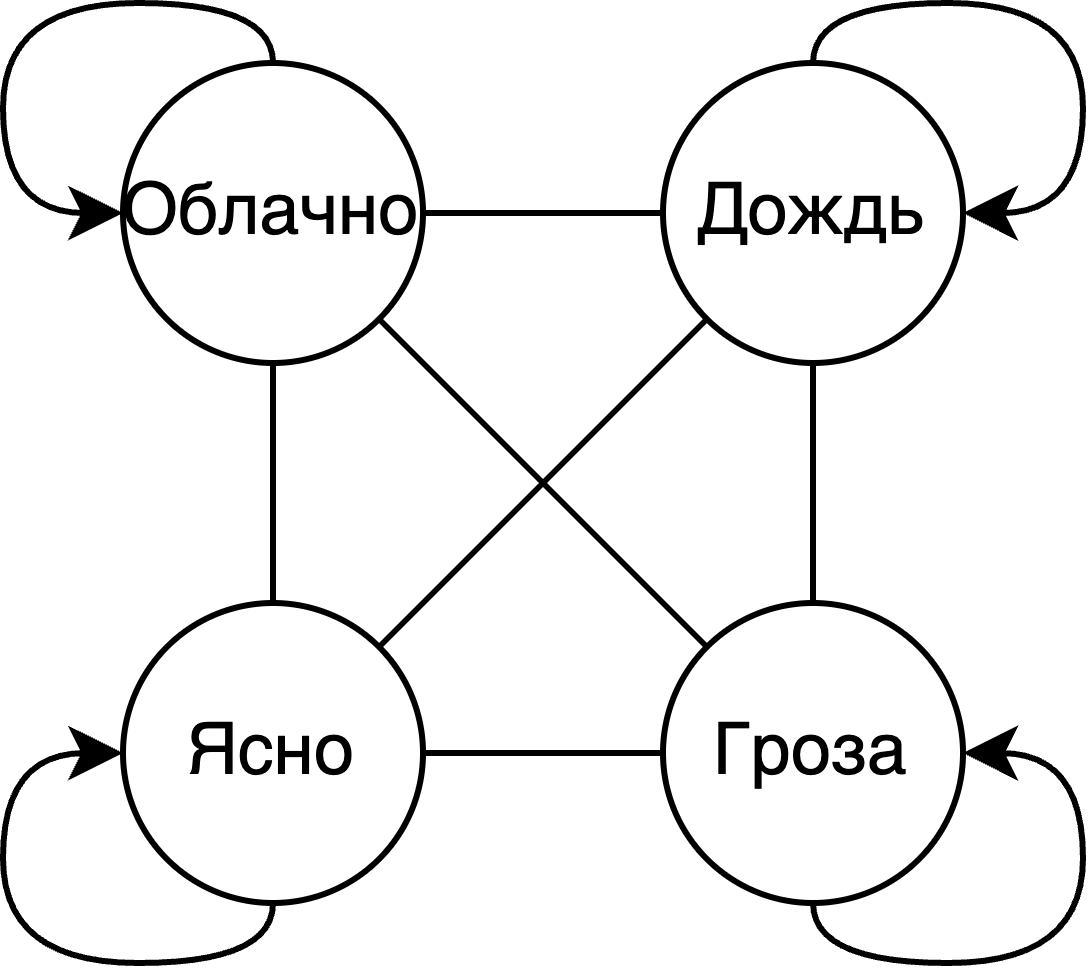
\includegraphics[width=0.40\linewidth]{src/img/1/pogoda_state_machine.png}
		\caption{Конечный автомат для примера прогнозирования погоды}
		\label{fig:pogoda_state_machine}
	\end{center}
\end{figure}

Давайте рассмотрим вероятность наблюдения последовательности событий $q_{i,1}, q_{i,2}, \ldots, q_{i,k}$, при условии начального состояния $a_o$. Эта вероятность определяется как произведение вероятностей каждого отдельного события: $P(q_{i,1}, q_{i,2}, \ldots, q_{i,k}) = a_o \cdot a_{i,1} \cdot a_{i,2} \cdot \ldots \cdot a_{i,k}$.

В частности, для вычисления вероятности того, что объект останется в состоянии $q_i$ в течение $d$ временных интервалов подряд, используется формула: $P(d_i) = a_{ii}^{d-1} \cdot (1 - a_{ii})$.

Математическое ожидание времени пребывания объекта в состоянии $q_i$ в течение $d$ временных интервалов подряд выглядит следующим образом:

$$E[ P(D) ] = \sum\limits_i d_i \cdot P(d_i) = \sum\limits_i d_i \cdot a_{ii}^{d-1} \cdot (1 - a_{ii}) = \dfrac{1}{1 - a_{ii}}$$.

Это выражение показывает, что математическое ожидание времени пребывания объекта в состоянии $q_i$ зависит только от вероятности перехода из этого состояния в другое.

В реальных приложениях, чтобы оценить априорные вероятности и вероятности перехода в марковских цепях, используют собранные данные или наблюдаемые значения. Эти оценки позволяют создать эмпирическую основу для модели. Оценка априорных вероятностей предполагает нахождение частоты каждого состояния в общем наборе данных. Априорная вероятность состояния $q_i$, обозначенная как $\pi_i$, рассчитывается как отношение числа наблюдений состояния $q_i$ к общему количеству наблюдений. Это выражается следующим образом: $\pi_i = \gamma_{0, i} / N$, где $N$ - общее количество наблюдений, а $\gamma_{0, i}$ - количество раз, когда наблюдалось состояние $q_i$. Таким образом, эта вероятность отражает базовую вероятность нахождения системы в каждом из возможных состояний. Вероятности перехода, определяющие вероятность перехода из одного состояния в другое, также оцениваются на основе наблюдаемых данных. Чтобы найти вероятность перехода из состояния $q_i$ в состояние $q_j$, используют следующий подход: делят число переходов из $q_i$ в $q_j$ на общее количество переходов из $q_i$. Формально, вероятность перехода $a_{ij}$ можно выразить как: $a_{ij} = \gamma_{ij} / \sum\limits_{j = 1}^n \gamma_{ij}$, где $\gamma_{ij}$ - количество наблюдений перехода из состояния $q_i$ в состояние $q_j$, а $\sum_{j = 1}^n \gamma_{ij}$ - общее число переходов из состояния $q_i$. Этот метод позволяет оценить вероятности переходов, основанные на фактических наблюдениях, что является ключевым шагом в построении марковских моделей.

Описанная выше модель марковских цепей предполагает, что все состояния системы можно наблюдать и точно измерить на каждом шаге времени. Однако в реальных приложениях это предположение часто не соответствует действительности. Например, в задачах прогнозирования погоды непосредственное наблюдение состояния атмосферы является сложной задачей, поскольку это состояние оценивается на основе множества показателей, полученных с различных датчиков. В таких случаях, когда прямое наблюдение состояния невозможно или неполно, применяется концепция скрытых марковских цепей.

Скрытые марковские цепи (Hidden Markov Models, HMM) расширяют традиционную марковскую цепь, вводя разделение между "скрытыми" и "наблюдаемыми" состояниями. В этой модели состояния системы по-прежнему определяются марковским свойством, где вероятность перехода из одного состояния в другое зависит только от текущего состояния. Однако теперь эти состояния недоступны для прямого наблюдения. Вместо этого у нас есть наблюдаемые данные, которые дают информацию о состоянии, но не напрямую.

Для описания связи между скрытыми и наблюдаемыми состояниями вводится дополнительный параметр, который характеризует вероятность получения наблюдаемого результата, исходя из скрытого состояния. Этот параметр, обозначаемый как $P(O_t | S_t)$, определяет вероятность наблюдения $O_t$ при условии, что система находится в скрытом состоянии $S_t$. Использование этого параметра позволяет моделировать связь между измеряемыми данными и внутренними состояниями системы, которые не видны напрямую.

Таким образом, в скрытых марковских цепях есть два ключевых аспекта:

\begin{itemize}
	\item переходы между скрытыми состояниями — как в традиционной марковской цепи, они задаются матрицей переходов, которая определяет вероятность перехода из одного скрытого состояния в другое;
	\item вероятность наблюдения — этот параметр определяет, насколько вероятно получить конкретное наблюдение, исходя из скрытого состояния.
\end{itemize}

Скрытые марковские цепи широко используются в различных областях, где наблюдаемые данные могут не отражать напрямую внутренние состояния системы, такие как обработка речи, биоинформатика, финансовый анализ и другие.




\subsection{Марковские случайные поля}






\subsection{Байесовские сети}




\section{Модели принятия решений}



\subsection{Графы принятия решений}





\section{Интеллектуальный анализ с помощью теории графов}



\section{Варианты хранения взаимосвязанных данных}



\section{Моделирование данных графами}



\section{Внутреннее устройство графовых баз данных}






